\documentclass[11pt]{article}

\usepackage{nmrdoc}
\usepackage{siunitx}
\usepackage{bm}
\usepackage{tikz}

\sisetup{per-mode=symbol}
\DeclareSIUnit{\angstrom}{\text{\AA}}
\DeclareSIUnit{\elementarycharge}{e}

\newcommand{\code}[1]{\texttt{#1}}
\setlength{\parindent}{0pt}
\setlength{\parskip}{0.42em}
\emergencystretch=3em

\begin{document}
\NmrTitle{Numerical Addendum: HydrationShell Calculator}

This calculator does not run a factorization, a quadrature rule, a tensor
projection, or a spatial query over waters. The implementation uses direct
loops over explicit waters and ions: one squared-distance shell gate, one sign
test against a reference direction, one water-dipole direction-cosine average,
and a nearest-ion minimum. The sibling \code{HydrationGeometryResult} uses the
same first-shell water scan but takes its reference direction from the
solvent-accessible surface area (SASA) normal, sums first-shell water dipoles,
and derives alignment and coherence from that sum. The listings below are
distilled from the source --- loops and bookkeeping trimmed --- but the
constants, guards, inequalities, and output shapes are the implementation's.

\section{Candidate enumeration}

The applied-maths inventory lists nanoflann k-d trees as the shared spatial
query mechanism. This pair of classes does not use a water k-d tree. The
\code{HydrationShellResult} header declares \code{SpatialIndexResult} as a
pipeline dependency, but \code{Compute()} never reads it; \code{SpatialIndexResult}
itself builds trees over protein atom positions, ring centres, and bond
midpoints, not over \code{SolventEnvironment::water\_O\_positions}. The water
part of the calculator is therefore an all-waters scan for every protein atom.
The ion part is an all-ions scan for every protein atom. For \(N\) protein atoms,
\(W\) waters, and \(I\) ions, the work in these two loops is \(O(NW+NI)\) per
frame.

The first-shell gate is a squared-distance comparison. For atom \(i\) at
\(\bm r_i\) and water oxygen \(w\) at \(\bm o_w\), \code{r} is
\(\bm o_w-\bm r_i\) and \code{d\_sq} is \(|\bm r|^2\). The configured cutoff is
\code{water\_first\_shell\_cutoff}, \(\SI{3.5}{\angstrom}\) in
\code{data/calculator\_params.toml}. Since the code continues only when
\code{d\_sq > first\_sq}, a water exactly on the cutoff remains in the shell.
There is no radial histogram and no second shell in these classes.

\begin{codebox}
const double first_shell_cutoff =
    CalculatorConfig::Get("water_first_shell_cutoff");
const double first_sq = first_shell_cutoff * first_shell_cutoff;

for (size_t ai = 0; ai < N; ++ai) {
    Vec3 pos_i = conf.AtomAt(ai).Position();

    for (size_t wi = 0; wi < W; ++wi) {
        Vec3 r = solvent.waters[wi].O_pos - pos_i;  // atom -> oxygen
        double d_sq = r.squaredNorm();
        if (d_sq > first_sq) continue;              // accepts d <= cutoff

        double d = std::sqrt(d_sq);
        Vec3 r_hat = r / d;
        ...
    }
}
\end{codebox}

The shell gate depends only on the oxygen position. Hydrogen positions enter
only through water dipoles after the oxygen has passed the gate. The
normalisation \code{r / d} has no zero-distance guard; a selected water oxygen
exactly coincident with the target atom is outside the guarded cases in this
path.

\section{Centroid half-shell and water dipoles}

\code{HydrationShellResult} first forms \code{protein\_com}, but the number is a
coordinate centroid, not a mass centre:
\[
  \bm c = \frac{1}{N}\sum_{j=1}^N \bm r_j .
\]
For each atom, \code{to\_interior} is
\(\hat{\bm u}_i=(\bm c-\bm r_i)/|\bm c-\bm r_i|\), the centroid-facing reference
direction. A first-shell water is buried when
\(\hat{\bm r}_{iw}\cdot\hat{\bm u}_i>0\). The equality case goes to exposed,
because every non-positive value follows the \code{else} branch. The
normalisation of \(\bm c-\bm r_i\) is also unguarded; an atom exactly at the
coordinate centroid is outside the guarded cases in this path.

\begin{codebox}
Vec3 protein_com = Vec3::Zero();
for (size_t i = 0; i < N; ++i)
    protein_com += conf.AtomAt(i).Position();
protein_com /= static_cast<double>(N);

Vec3 to_interior = (protein_com - pos_i).normalized();

int n_exposed = 0, n_buried = 0;
double dipole_cos_sum = 0.0;
int dipole_count = 0;

double cos_interior = r_hat.dot(to_interior);
if (cos_interior > 0)
    ++n_buried;
else
    ++n_exposed;

Vec3 dipole = solvent.waters[wi].Dipole();
double dip_mag = dipole.norm();
if (dip_mag > CalculatorConfig::Get("near_zero_vector_norm_threshold")) {
    dipole_cos_sum += dipole.dot(r_hat) / dip_mag;
    ++dipole_count;
}
\end{codebox}

The half-shell output is an exposed-side fraction, not a signed centred
asymmetry:
\[
  h_i =
  \begin{cases}
  n_{\mathrm{exposed}}/(n_{\mathrm{exposed}}+n_{\mathrm{buried}}),
    & n_{\mathrm{exposed}}+n_{\mathrm{buried}}>0,\\
  0, & n_{\mathrm{exposed}}+n_{\mathrm{buried}}=0 .
  \end{cases}
\]
The first-shell count itself is not written by \code{HydrationShellResult}, so
\(h_i=0\) can mean either no first-shell water or all counted waters on the
buried side.

\code{WaterMolecule::Dipole()} returns
\[
  \bm\mu_w =
  q_{\mathrm H}(\bm h_{1w}-\bm o_w)
  +q_{\mathrm H}(\bm h_{2w}-\bm o_w),
\]
because the oxygen is the origin of the water-local displacement sum. The
coordinates are in \(\si{\angstrom}\) and the charges in
\(\si{\elementarycharge}\). Thus \(\bm\mu_w\) is in
\(\si{\elementarycharge\angstrom}\).

For the HydrationShell dipole channel, each accepted water contributes only the
direction cosine
\(\bm\mu_w\cdot\hat{\bm r}_{iw}/|\bm\mu_w|\). Waters whose dipole magnitude is
not greater than \code{near\_zero\_vector\_norm\_threshold},
\(10^{-10}\), still count in the half-shell fraction but do not enter this
average.
If no water contributes to the dipole average, the output is zero.

\begin{center}
\centering
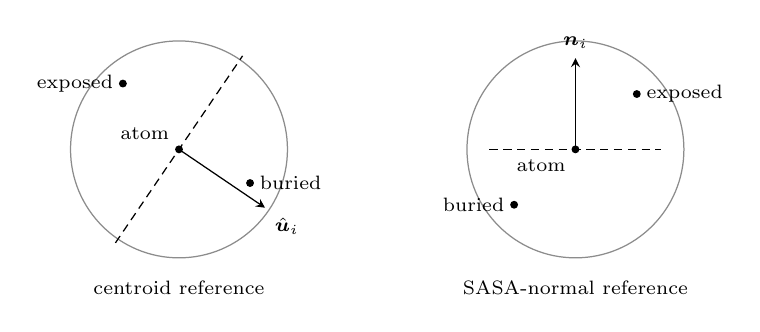
\begin{tikzpicture}[scale=0.95,line width=0.45pt,>=stealth]
  \coordinate (A) at (0,0);
  \draw[black!45] (A) circle (1.45);
  \draw[densely dashed] (-0.85,-1.25) -- (0.85,1.25);
  \draw[->] (A) -- (1.15,-0.78) node[below right] {\scriptsize \(\hat{\bm u}_i\)};
  \fill (A) circle (1.5pt) node[above left] {\scriptsize atom};
  \fill (0.95,-0.45) circle (1.5pt) node[right] {\scriptsize buried};
  \fill (-0.75,0.88) circle (1.5pt) node[left] {\scriptsize exposed};
  \node at (0,-1.85) {\scriptsize centroid reference};

  \begin{scope}[xshift=5.3cm]
    \coordinate (B) at (0,0);
    \draw[black!45] (B) circle (1.45);
    \draw[densely dashed] (-1.15,0) -- (1.15,0);
    \draw[->] (B) -- (0,1.22) node[above] {\scriptsize \(\bm n_i\)};
    \fill (B) circle (1.5pt) node[below left] {\scriptsize atom};
    \fill (0.82,0.74) circle (1.5pt) node[right] {\scriptsize exposed};
    \fill (-0.82,-0.74) circle (1.5pt) node[left] {\scriptsize buried};
    \node at (0,-1.85) {\scriptsize SASA-normal reference};
  \end{scope}
\end{tikzpicture}

\smallskip
{\small\textbf{Figure.} Each panel shows a first-shell ball cut by a plane
through the atom.
The centroid-reference panel counts the positive side of \(\hat{\bm u}_i\) as
buried; the SASA-normal panel counts the positive side of \(\bm n_i\) as
exposed.}
\end{center}

\section{Nearest ion}

The nearest-ion channel is another direct scan. For each ion \(k\), the code
computes \(|\bm z_k-\bm r_i|\) in \(\si{\angstrom}\). The stored best value
changes only when the new distance is strictly smaller than the current best, so
an exact tie keeps the earlier ion in storage order. After the scan, the cutoff
test is also strict: an ion at exactly \code{hydration\_ion\_cutoff},
\(\SI{20.0}{\angstrom}\), is reported as absent.

\begin{codebox}
double best_ion_dist = std::numeric_limits<double>::max();
double best_ion_charge = 0.0;

for (size_t ii = 0; ii < solvent.IonCount(); ++ii) {
    double d = (solvent.ions[ii].pos - pos_i).norm();
    if (d < best_ion_dist) {
        best_ion_dist = d;
        best_ion_charge = solvent.ions[ii].charge;
    }
}

atom.nearest_ion_distance =
    (best_ion_dist < ion_cutoff)
    ? best_ion_dist : std::numeric_limits<double>::infinity();
atom.nearest_ion_charge =
    (best_ion_dist < ion_cutoff) ? best_ion_charge : 0.0;
\end{codebox}

With solvent present but no ions, \code{best\_ion\_dist} stays at the largest
finite double, fails the strict cutoff, and the same absent record is written:
\(+\infty\) for distance and zero for charge. The zero charge is interpretable
only with the distance channel; it is also the absent sentinel.

\section{SASA-normal hydration geometry}

\code{HydrationGeometryResult} keeps the same first-shell oxygen gate and the
same all-waters scan, but it consumes a different reference vector:
\code{atom.sasa\_normal}, already written by \code{SasaResult}. This class does
not recompute the sampled SASA normal; it copies the stored vector to
\code{water\_surface\_normal} and uses its sign in the half-shell split. When
the normal norm is not greater than \code{near\_zero\_vector\_norm\_threshold},
all first-shell waters count as exposed. When the normal is present,
\(\hat{\bm r}_{iw}\cdot\bm n_i>0\) is exposed and the equality case is buried.

\begin{codebox}
Vec3 normal = atom.sasa_normal;
atom.water_surface_normal = normal;

Vec3 dipole_sum = Vec3::Zero();
int n_exposed = 0, n_buried = 0, n_shell = 0;

for (size_t wi = 0; wi < W; ++wi) {
    Vec3 r = solvent.waters[wi].O_pos - pos_i;
    double d_sq = r.squaredNorm();
    if (d_sq > first_sq) continue;

    ++n_shell;
    dipole_sum += solvent.waters[wi].Dipole();

    double d = std::sqrt(d_sq);
    Vec3 r_hat = r / d;
    if (normal.norm() > near_zero) {
        double cos_normal = r_hat.dot(normal);
        if (cos_normal > 0) ++n_exposed;
        else                ++n_buried;
    } else {
        ++n_exposed;
    }
}
\end{codebox}

The net dipole \(\bm D_i=\sum_{w\in\mathcal W_i}\bm\mu_w\) keeps the
\(\si{\elementarycharge\angstrom}\) units of the water dipoles. No water is
removed from this vector sum by a near-zero dipole guard. Three scalar channels
are then derived from the same counts and vector:
\[
  h_i^{\mathrm{SASA}} =
  \frac{n_{\mathrm{exposed}}}
       {n_{\mathrm{exposed}}+n_{\mathrm{buried}}}
  \quad\hbox{when the denominator is nonzero,}
\]
\[
  a_i =
  \frac{\bm D_i\cdot\bm n_i}{|\bm D_i|\,|\bm n_i|},
  \qquad
  c_i = \frac{|\bm D_i|}{n_{\mathrm{shell}}}.
\]
The code writes zero for \(h_i^{\mathrm{SASA}}\) when no water is in the shell,
zero for \(a_i\) when either \(|\bm D_i|\) or \(|\bm n_i|\) is not greater than
the near-zero threshold, and zero for \(c_i\) when the shell is empty.
\code{sasa\_dipole\_alignment} is a cosine. \code{sasa\_dipole\_coherence} is
not dimensionless; it has units of \(\si{\elementarycharge\angstrom}\).

\begin{codebox}
atom.sasa_first_shell_count = n_shell;
atom.sasa_half_shell_asymmetry =
    (n_exposed + n_buried > 0)
    ? static_cast<double>(n_exposed) / (n_exposed + n_buried)
    : 0.0;

atom.water_dipole_vector = dipole_sum;

double dip_mag = dipole_sum.norm();
double norm_mag = normal.norm();
if (dip_mag > near_zero && norm_mag > near_zero)
    atom.sasa_dipole_alignment =
        dipole_sum.dot(normal) / (dip_mag * norm_mag);
else
    atom.sasa_dipole_alignment = 0.0;

atom.sasa_dipole_coherence =
    (n_shell > 0) ? dip_mag / static_cast<double>(n_shell) : 0.0;
\end{codebox}

\section{Output shapes}

No tensor is emitted by either class, so the shared
\code{SphericalTensor::Decompose} path is not used here. The values are scalars,
counts, and two three-vectors. They are solvent-geometry descriptors, not
shielding tensors and not chemical shifts.

\begin{codebox}
// hydration_shell.npy: (N, 4)
data[i*4 + 0] = a.half_shell_asymmetry;
data[i*4 + 1] = a.mean_water_dipole_cos;
data[i*4 + 2] = a.nearest_ion_distance;
data[i*4 + 3] = a.nearest_ion_charge;

// water_polarization.npy: (N, 10)
data[i*10 + 0] = a.water_dipole_vector.x();
data[i*10 + 1] = a.water_dipole_vector.y();
data[i*10 + 2] = a.water_dipole_vector.z();
data[i*10 + 3] = a.water_surface_normal.x();
data[i*10 + 4] = a.water_surface_normal.y();
data[i*10 + 5] = a.water_surface_normal.z();
data[i*10 + 6] = a.sasa_half_shell_asymmetry;
data[i*10 + 7] = a.sasa_dipole_alignment;
data[i*10 + 8] = a.sasa_dipole_coherence;
data[i*10 + 9] = static_cast<double>(a.sasa_first_shell_count);
\end{codebox}

The count in column 9 of \code{water\_polarization.npy} is stored as a double
because the NPY writer call emits a float64 matrix. The nearest-ion distance in
\code{hydration\_shell.npy} may be \(+\infty\). The code writes no explicit
boolean ion-present channel in this file.

\section{Glossary}

\textbf{First hydration shell.} A ball around a protein atom, populated by
water oxygens rather than by all water charge sites. A water with oxygen exactly
\(\SI{3.5}{\angstrom}\) from the atom is included by the squared-distance test;
its hydrogens then contribute only through the dipole vector. Formally, it is
\(\{w:|\bm o_w-\bm r_i|^2\le R_w^2\}\) with
\(R_w=\code{water\_first\_shell\_cutoff}\).

\textbf{Half-shell asymmetry.} A fraction made by cutting the first-shell ball
into two half-spaces through the atom and counting waters on one named side. In
\code{HydrationShellResult} the exposed side is the non-positive side of the
centroid-facing direction; in \code{HydrationGeometryResult} it is the positive
side of the SASA normal. If that normal's norm is not greater than the near-zero
threshold, all waters count as exposed. Formally, it is \(n_{\mathrm{exposed}}/
(n_{\mathrm{exposed}}+n_{\mathrm{buried}})\), with zero written for an empty
denominator.

\textbf{Water dipole vector.} The arrow from the water oxygen toward the
charged hydrogen side, scaled by the topology hydrogen charge and the O--H
geometry. For a three-site water with topology hydrogen charge \(q_{\mathrm H}\),
the vector is the sum of the two charged O--H displacements, in
\(\si{\elementarycharge\angstrom}\). Formally,
\(\bm\mu_w=\sum_j q_j(\bm r_j-\bm o_w)\), with the oxygen term zero in the
stored origin.

\textbf{SASA normal.} The outward direction already estimated by the SASA
calculator: it averages the unit directions of the non-occluded test points on
an expanded atom sphere and normalises the sum when that sum is above the
near-zero threshold. If the stored normal's norm is not above that threshold,
HydrationGeometry then takes the no-direction branch.
Formally, this calculator consumes \(\bm n_i=\code{atom.sasa\_normal}\) as
stored; it does not rebuild the Fibonacci-lattice sampling and occlusion test
that produced it.

\end{document}
